% mn2esample.tex
%
% v2.1 released 22nd May 2002 (G. Hutton)
%
%
% Previous versions of this sample document were
% compatible with the LaTeX 2.09 style file mn.sty
% v1.2 released 5th September 1994 (M. Reed)
% v1.1 released 18th July 1994
% v1.0 released 28th January 1994

\documentclass[useAMS,usenatbib]{mn2e}
\usepackage{graphicx}
%\usepackage{aas_macros}
\usepackage{multirow}
\usepackage{hyperref}


% If your system does not have the AMS fonts version 2.0 installed, then
% remove the useAMS option.
%
% useAMS allows you to obtain upright Greek characters.
% e.g. \umu, \upi etc.  See the section on "Upright Greek characters" in
% this guide for further information.
%
% If you are using AMS 2.0 fonts, bold math letters/symbols are available
% at a larger range of sizes for NFSS release 1 and 2 (using \boldmath or
% preferably \bmath).
%
% The usenatbib command allows the use of Patrick Daly's natbib.sty for
% cross-referencing.
%
% If you wish to typeset the paper in Times font (if you do not have the
% PostScript Type 1 Computer Modern fonts you will need to do this to get
% smoother fonts in a PDF file) then uncomment the next line
% \usepackage{Times}

%%%%% AUTHORS - PLACE YOUR OWN MACROS HERE %%%%%


%%%%%%%%%%%%%%%%%%%%%%%%%%%%%%%%%%%%%%%%%%%%%%%%

\title[Deconstructing M83]{Deconstructing a galaxy: identifying components of M83 with photometric clustering}
\author[Barmby \& Kiar]
{
P. Barmby$^{1}$\thanks{E-mail: pbarmby@uwo.ca} and 
A.K. Kiar$^{1}$\\
$^{1}$Department of Physics and Astronomy, University of Western Ontario, London, ON, N6A 3K7, Canada\\
%$^{2}$address 2
}

\begin{document}

\date{}

%\pagerange{\pageref{firstpage}--\pageref{lastpage}} \pubyear{2002}

\maketitle

\label{firstpage}

\begin{abstract}
%\input{abs}
\end{abstract}

\begin{keywords}
keywords here
\end{keywords}

\section{Introduction}

\section{Introduction}


%\item Galaxies have a lot of discrete sub-components: stars, clusters, nebulae, nucleus.
Galaxies are complex systems, comprised of numerous components with an enourmous range of size,
mass, density, and composition.
These components can be divided into baryonic (stars and their remnants,
nebulae, star clusters, nucleus) and non-baryonic (dark matter);
cataloging the components and describing
the interactions between them is a key step in elucidating the natural history of galaxies.
Only in nearby galaxies can individual sub-components be resolved.
As observational technology has advanced,
the definition of ``nearby'' has changed and will continue to do so, from Milky Way satellites and Local Group galaxies, to a few
Megaparsecs \citep[distance at which stars can be resolved with HST][]{},
to XX Mpc \citep[distance at which stars can be resolved with JWST][]{},
to the entire observable universe with potential future facilities \citep{}.

%\item One way to isolate specific components is with narrow-band filters or CMD analysis.
What is the most efficient way to survey the sub-components of a nearby galaxy?
Here we are discussing components detectable in imaging at ultraviolet through infrared wavelengths,
i.e. with effective temperatures in the range XX--XX~K.
Much cooler or hotter types of objects (molecular gas, accreting compact objects) are better-detected at other wavelengths.
Particular stellar types, or star clusters, are often identified with broad-band colour-magnitude diagrams \citep[e.g.][]{}.
Narrow-band filters can also isolate special stellar types \citep[e.g.][]{} or objects prominent in emission
lines such as planetary nebulae or supernova remnants \citep[e.g.][]{}.
Observations are typically designed with detection of particular classes in mind and sometimes re-used for additional purposes \citep[e.g.][]{}.
Spectroscopic follow-up is often required to confirm candidates.
New observational facilities which provide spatially-resolved spectroscopy  \citep[e.g.]{}{} may reduce the need for separate imaging and follow-up steps,
but greatly increase the complexity of initial data analysis.


Multi-wavelength surveys are extremely common in studies of unresolved galaxies in the distant universe.
While these are often designed to select galaxies or active galactic nuclei with specific properties \citep[e.g.][]{},
sometimes they are pure blank-field surveys.
Broadband ($R=\Delta \lambda/\lambda \lesssim X$) filters are the most common imaging modality,
although there have been a few attempts at narrow- or medium-band surveys as well \citep[e.g.][]{combo-17},
Clustering in colour space can be used to select particular classes of objects from a survey,
for example in selecting AGN via mid-infrared colours \citep[e.g.][]{},
or high-redshift galaxies via Lyman-break dropouts \citep[e.g.][]{}. 
{\bf give some examples here of sophisticated analysis of colour spaces.}

%\item But what if you already have all the filters, and you want to make a census? 
%Can start with properties of known classes of objects \& pick out from multi-dimensional dataset.
%\item Another approach is to see what blind clustering gets you: how many groups and what are they?
%How does this depend on the (number of) wavelengths used?
The purpose of this work is to treat a nearby galaxy as if it were a blank field for surveys, and investigate the
usefulness of different photometric colours for identifying sub-components.
We make use of the Early Release Science (ERS) observations with the Wide-Field Camera 3 (WFC3) of the nearby spiral galaxy M83 \citep{}
and in particular the catalog of point sources produced by \citet{}.
We form colours from the photometric measurements in the catalog and apply several clustering techniques to two-colour datasets.
In conjunction with published catalogs of galaxy components, we identify the optimum parameters for clustering such a photometric dataset,
and the best choices of filter.




%Outline of intro:
%
%\begin{enumerate}
%\item Galaxies have a lot of discrete sub-components: stars, clusters, nebulae, nucleus.
%\item One way to isolate specific components is with narrow-band filters or CMD analysis.
%\item But what if you already have all the filters, and you want to make a census? Can start
%with properties of known classes of objects \& pick out from multi-dimensional dataset.
%\item Another approach is to see what blind clustering gets you: how many groups and what are they?
%How does this depend on the (number of) wavelengths used?
%\end{enumerate}
%
%Work to be cited: 
%\begin{itemize}
%\item astro applications of k-means clustering 
%\item astro applications of other ML techniques
%\item general bkg on galaxy constituents
%\item ??
%\end{itemize}


\section{Data}
\section{Data}

%\item intro to M83: global parameters (distance, size, environment)
The dataset used for this study is the Wide-Field Camera-3
Early Release Science (ERS) observations of the nearby spiral galaxy Messier 83 (M83).
M83 is a grand-design spiral of type SAB, located at a distance of 4.66~Mpc \citep{tully13}
and the largest member of the M83 subgroup of the nearby Centaurus group of galaxies \citep{tully15}.
The galaxy's apparent radius of $\sim12$~arcmin \citep{} is reasonably well-matched to the camera's field of view (XX true? XX)
{\bf And here we note some other interesting things about M83.}

%\item Intro to WFC3 ERS dataset
%\item existing studies with this dataset (cluster, massive stars, etc)
% ref: chandar10, section. TODO: check for (unintentional!) plagiarism
The objective of the ERS observations as a whole was to probe star formation in galaxies.
The observations of M83 were made in broad- and narrow-band filters in order to characterize both stellar and nebular properties.
They cover a $3.6\times3.6$~kpc$^2$ region in the northern portion of the galaxy, including the nucleus,
a portion of a spiral arm and an interarm region.
The spatial resolution of the images is $0\farcs0396$~arcsec~pixel$^{-1}$,
corresponding to a linear scale of $XX$~pc~pixel$^{-1}$ at the 4.66~Mpc distance.
A complete description of the observations and data processing is given by \citet{chandar10};
our work here uses the observations in the UVIS channel, listed in Table~\ref{tab:filters}.
A number of previous studies have used the ERS M83 dataset for various purposes.
These include studies of 
star clusters \citep{chandar10, wofford11, whitmore11, bastian11, bastian12, fouesneau12, silva13, andrews14, chandar14, adamo15,ryon15,hollyhead15, sun16},
H~{\sc ii} regions \citep{liu13}, supernova remnants and the interstellar medium \citep{dopita10, hong11, blair14, blair15}, 
resolved stars \citep{kim12, williams15},
and a super-Eddington off-nuclear black hole \citep{soria14}.


\begin{table}
\centering
\caption{
\label{tab:filters}}
\begin{tabular}{lll}
\hline\hline
Filter & Name & Exposure time\\
\hline
F225W &  Wide UV & 1800~s\\
F336W &  $U$-band & 1890~s\\ 
%F373N &  [\ion{O}{iii}] & 2400~s\\
F438W &  $B$-band & 1180~s\\
F487N &  H$\beta$ & 2700~s\\
%F502N &  [\ion{O}{ii}] & 2484~s
F555W &  V-band, South field & 1203~s\\
%F547M &  V-band, North field & \\
%F657N &  H$\alpha$+[\ion{N}{ii}]& 1484~s\\ 
%F673N &  [\ion{S}{ii}] & 1850~s\\
F814W &  $I$-band & 1203~s\\
\hline
\end{tabular}
\end{table}

We analyze the catalog produced by \citet{chandar10} and made available via **REF**.
The objects in this catalog were detected on a `white-light' image produced by a weighted combination of the $UBVI$ images.
Photometry in 0.5- and 3-pixel radius apertures at the positions of the detected sources was performed on the broad- and narrow-band images and tabulated in the Vega magnitude system. %TODO: pick one of the 2 apertures and just use that. AK: ideas on which one?
We apply the correction to the F657N magnitude zeropoint (from 20.72 to 22.35) noted in the header of the catalog.
\citet{chandar10} discussed aperture corrections for this catalog, but since we are primarily concerned with colours,
we omit any aperture corrections. %TODO: make sure this is a good idea.
The catalog contains about 68000 objects which are expected to include individual stars, star clusters,
supernova remnants, H${\sc ii}$ regions, planetary nebulae, %TODO: check that we expect these to be detectable!
stellar blends, and background galaxies. % TODO: anything else?
Completeness and reliability of the catalog are not discussed by \citet{chandar10},
but a visual inspection of the the detected sources on the white-light image suggests that %TO BE COMPLETED..
XX objects are flagged in the catalog as being problematic %TODO: AK please compute this number using flag column
and we remove them from our analysis.

Table~\ref{tab:cat_numbers} and Figure~\ref{fig:mag_unc} characterize the catalog in terms of measurements in individual filters.
Not all objects are detected in all filters;
Table~\ref{tab:cat_numbers} gives the number of objects for which photometry is reported in a given filter,
the number for which reported magnitude uncertainty is $0.2$~mag or less,
and the aperture magnitude at which the median magnitude uncertainty is $0.2$~mag. 
%TODO: think about whether 0.2 is the right number.
% Catalog header says ``The  errors are probably reasonable but have not been "normalized" to truth (by comparing  subexposures), so not recomm ended for use except in a relative scale.'' Chandar paper does not discuss mag uncertainties.
Figure~\ref{fig:mag_unc} shows the distributions of magnitudes and uncertainties in the individual filters.

%AK: please calculate numbers here. For the last column scipy.stats.binned_statistic is a good way to do this.
\begin{table}
\centering
\caption{
\label{tab:cat_numbers}}
\begin{tabular}{lrrlr}
\hline\hline
Filter & $N_{\rm obj}$ & $N_{\rm good}$ & $m_{\rm good}$ & $N_{\rm X-555}$\\
\hline
F225W &  N & N & m & N\\
F336W &  N & N & m & N\\
F373N &  N & N & m & N\\
F438W &  N & N & m & N\\
F487N &  N & N & m & N\\
F502N &  N & N & m & N\\
F555W &  N & N & m & N\\
F657N &  N & N & m & N\\
F673N &  N & N & m & N\\
F814W &  N & N & m & N\\
\hline
\end{tabular}
\end{table}

%AK: here's where the plots go.
\begin{figure*}
\centering
%\includegraphics{fig1}
\caption{Distribution of magnitudes and uncertainties for objects in the \citet{chandar10} M83 ERS catalog.}
\label{fig:mag_unc}
\end{figure*}

% TODO: discuss (this might also go in a different section)
Our analysis in this paper is primarily concerned with colours, rather than luminosities.
Uncertainties in colours are computed as the quadrature sum of the relevant magnitudes.
Observations in 10 bands allow the generation of 45 different colours,
but not all of these colours are likely to be useful in characterizing components of the galaxy.
As the F555W band has the most individual detections, %TODO: AK: is this true?
we initially compute colours relative to this band.
The last column of Table~\ref{tab:cat_numbers} gives the number of objects for which a `good' colour (uncertainty $<0.2$~mag) is available.
%TODO: may use different number than 0.2.



%Outline for data section
%%\begin{enumerate}
%\item Intro to WFC3 ERS dataset
%\item intro to M83: global parameters (distance, size, environment)
%\item existing studies with this dataset (cluster, massive stars, etc)
%\item description of catalog (is there a ref for this??)
%\item anything about these data we don't like/didn't use?

%\end{enumerate}



\section{Analysis}
% Analysis section
In this section we will outline the process used for each of the clustering methods.
An aim of this work was to help astronomers determine which filters were best at identifying different types of objects in a survey. 
Since the average survey is limited to four filters, different combinations of four filters were used to construct colours for clustering. 
Colours were constructed using the difference between two wavelengths. For a given combination of four filters, all possible colour combinations were used. % Change as needed
The feature space was constructed in two and three dimensions, to add a layer of analysis that isn't typically found in colour-colour space.

\subsection{Clustering Process}
Clustering was performed using all three methods for each colour combination. 
The methods were used independantly and in unison in order to determine the optimal clustering.
The following process allowed the investigation of the effect of all paramters on each clustering technique, leading to an optimal clustering. 
\begin{enumerate}
\item \textbf{Mean-Shift:} Mean-Shift clustering was performed first by estimating the bandwidth paramter with the $estimate_bandwidth$ function in $scikit_learn$.
Following the initial clustering, a "bandwidth hierarchy" was created by performing the clustering again with bandwidth values between $\pm$ intervals of $0.1$ from the estimated bandwidth.

\item \textbf{AP:} Affinity Propagation clustering was then performed by setting the preferences to 10\% of the number of objects in the data set, and setting the damping factor to $0.95$.
Following that clustering, an "Affinity hierarchy" was created by varrying the damping factor, and preference value to determine the effect of each parameter. 

\item \textbf{K-Means:} K-Means clustering was performed last.
The first two clusterings were performed using the number of clusters determined from the initial clusterings by Mean-Shift and AP.
Next, K-Means was performed with $K = \pm 4$ from the original clustering. 
\end{enumerate}
\subsection{Selecting the Clustering}
In order to determine the optimal clustering, a series of metrics were used.
For each clustering, the silhouette score, cluster centers, root mean square, average and standard devation of each colour, and the distances between points in each cluster were calculated. 
\subsubsection{Silhouette Score}
The silhouette score is a metric used to describe the compactness of a cluster in a given clustering and is calculated as an average of all samples in a clustering.  
The silhouette score is given by:
\begin{equation}
\label{eq:ss}
Silhouette Score = \frac{b - a}{\textit{max}\big(a, b\big)}
\end{equation}
where $a$ is the mean intra-cluster distance, and $b$ is the distance between a point and the nearest cluster that point is not a member of.
In addition to the average score of the clustering, the average score for each cluster within the clustering was computed.
The cluster score determines what is driving the average score, and uncovers which clusters are most compact.

\subsubsection{Cluster Statistics}
Various statistics were calculated for each cluster within a clustering to help describe the similarity between the objects in a given cluster.
The standard deviation and average colour was calculated for each colour and each cluster within a clustering. 
These metrics describe the distribution of the objects in the colour-colour space within a cluster. 
Clusters that had large standard deviations were viewed as too dissimilar to be a meaningful cluster, and the clustering parameters were changed or the clustering was removed. 
Clusters whose averages and medians were not close were also discredited. 

The fractional sizes of each cluster were also calculated.
This metric describes the distribution of objects between clusters, and provided a complete way to evaluate a given clustering. 
If a clustering segmented the objects into a large cluster followed by several smaller ones, the clustering was investigated further, as this segmentation could mean one of two things. 
This type of clustering could be a result of the identification of interesting objects, in which case the clustering algorithm was able to identify the objects and place them in the same cluster.
However, this type of clustering could also be a result of the underlying distribution of the data, as the clustering techniques are largely drawn to areas of high density.
If this is the case, the clustering only created the smaller clusters as a result of the parameters imposed on the clustering.

\subsubsection{Parameter Relationships}
Aside from metrics, the relationships between various metrics were investigated to determine the optimal clustering.
Figure~\ref{fig:sscore} shows the relationship between the silhouette score and the number of clusters imposed on the data for each type of clustering. 
The optimal number of clusters is found where the relation flattens.
For K-Means, this point is between 5-10 clusters.
The Mean-Shift scores do not follow a similar distribution as K-Means, as the accuracy of Mean-Shift is more directly related to the bandwidth parameter, seen in Figure~\ref{fig:bwscore}.
\begin{figure*}
\centering
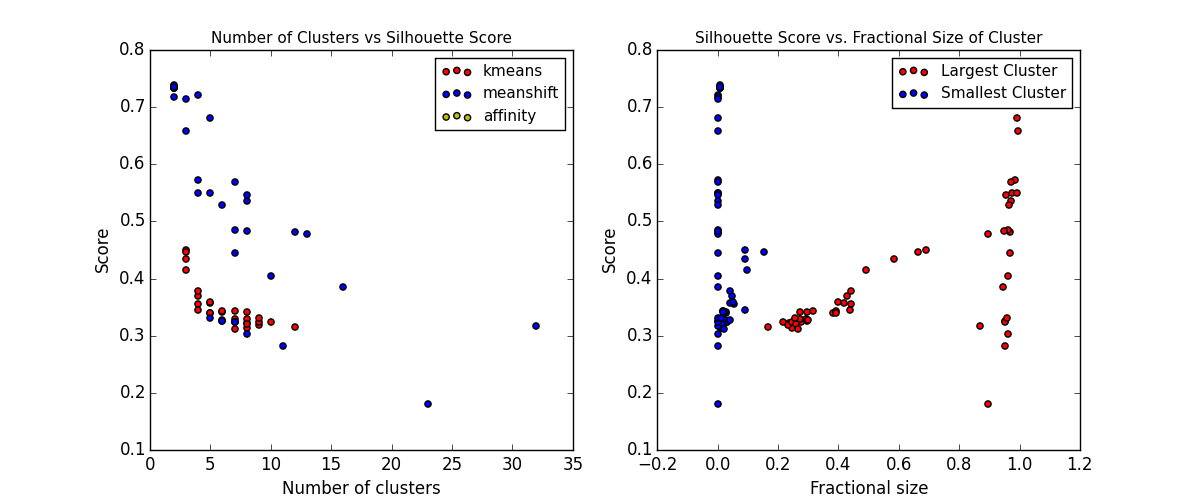
\includegraphics[width=0.5\textwidth]{figs/silhouette_score_relation}
\caption{Distribution of the silhouette score as a result of the number of clusters imposed. The \textit{blue} points are the scores of Mean-Shift clustering, \textit{red} points are scores of K-Means, and \textit{yellow} points are scores of AP.}
\label{fig:sscore}
\end{figure*}

\begin{figure*}
\centering
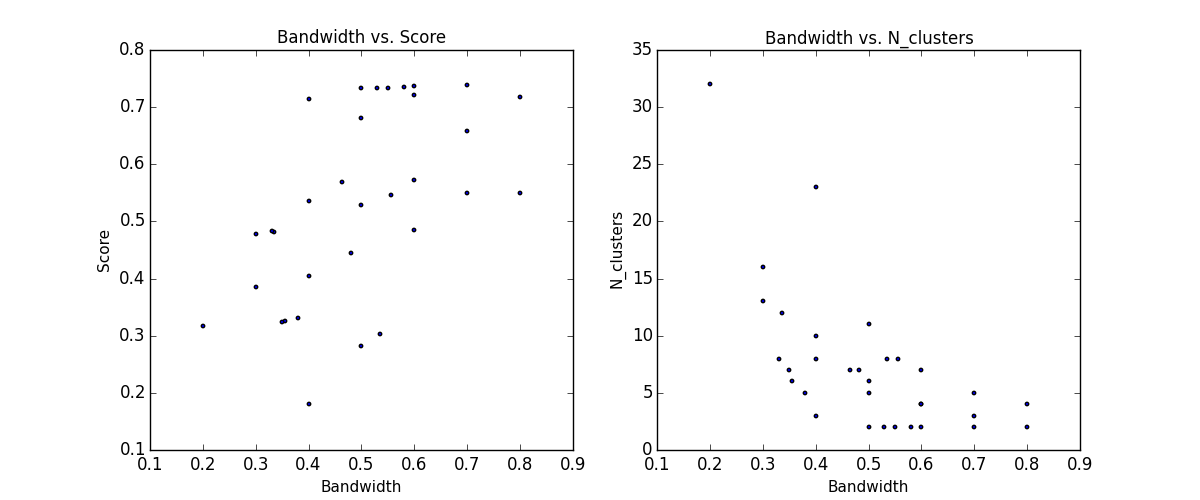
\includegraphics[width=0.5\textwidth]{figs/meanshift_parameters}
\caption{Distribution of the silhouette score as a function of bandwidth, and the distribution of the number of clusters as a function of bandwidth.}
\label{fig:bwscore}
\end{figure*}


\section{Results}
% Results section

\[ To be reorganized \]

The results of the analysis are grouped into the type of band used to make each colour.  % More general notes about results

\subsection{Broad \& Broad Band Combinations}

\subsection{Broad \& Narrow Band Combinations}
Each broad and narrow band combination was tested against every broad-broad band combination that did not boarder the narrow band.

\subsubsection{UVW - U}
The UVW - U combination was tested clustered with the B-I, V-I, and B-V colours. % More general information about what we are looking for in this combination

\paragraph{Mean-Shift}
When clustered using Mean-Shift, a similar pattern of clustering was seen in all combinations.
Due to the structure of the Mean-Shift algorithm, it is drawn towards areas of high density in the distribution. % Refernce meanshift paper
Since the distribution of the UVW-U combinations were generally consentrated around zero in the colour-colour space, the Mean-Shift algorithm would pick out one large cluster with many smaller ones. 
Each smaller cluster had to be investigated to determine if the algorithm had found a meaningful cluster, or if it had just clustered noise.
In order to determine this, a cluster hierarchy was created with different bandwidth values to see how long each cluster lasted in the bandwidth space. 
If a small cluster was created at a low bandwidth level and stayed alive until the number of clusters became 2-3, then it is reasonable to assume that the cluster was meaningful.
Figure ~\ref{fig:UVWMS1} shows the result of one trial of Mean-Shift clustering with $h=0.6$ which created 4 clusters. 
Figure ~\ref{fig:UVWMS2} shows the result of one trial of Mean-Shift clustering with $h=0.4$, creating 10 clusters. 
The structure of cluster $2$ in both Figure ~ref{fig:UVWMS1} and Figure ~ref{fig:UVWMS2} can be seen distinctly. 
This cluster would have been viewed as noise if the hierarchy was not created, but after testing multiple bandwidth values, it can be seen that these objects are significant. 

\begin{figure}[H]
\centering
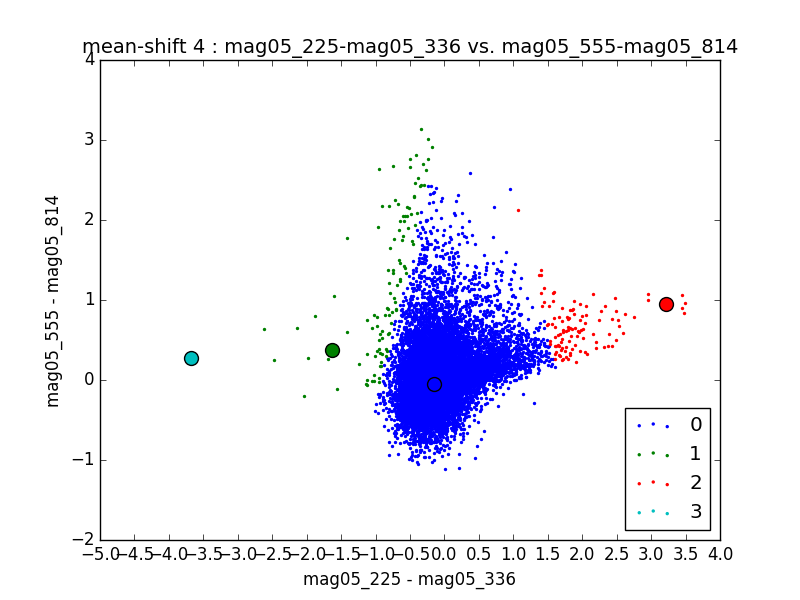
\includegraphics[width=\linewidth]{figs/meanshift_color_4cl_mag05_225-mag05_336vsmag05_555-mag05_814}
\caption{Colour-Colour distribution of the UVW-U and V-I colours, clustered using Mean-Shift with $h=0.6$. The colour of each point corresponds to the cluster the point was assigned to. Cluster numbers can be seen in the legend.}
\label{fig:UVWMS1}
\end{figure}

\begin{figure}[H]
\centering
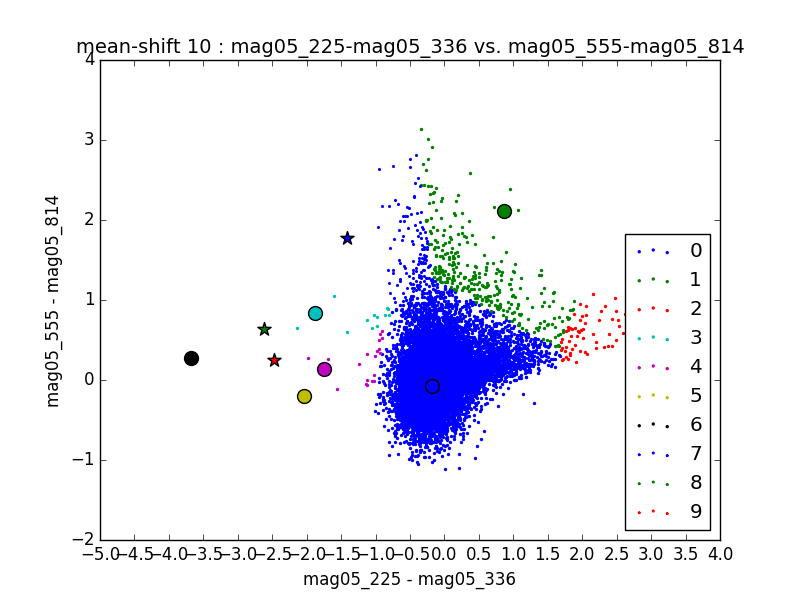
\includegraphics[width=\linewidth]{figs/meanshift_color_10cl_mag05_225-mag05_336vsmag05_555-mag05_814}
\caption{Colour-Colour distribution of the UVW-U and B-I colours, clustered using K-Means with $h=0.4$. The colour of each point corresponds to the cluster the point was assigned to. Cluster numbers can be seen in the legend.}
\label{fig:UVWMS2}
\end{figure}

\paragraph{K-Means}

When clustered using K-Means, two types of results were seen.
Figure ~\ref{fig:UVWKM1}, shows the result of K-Means clustering for $K=5$ against the B-V colour. 
\begin{figure}
\centering
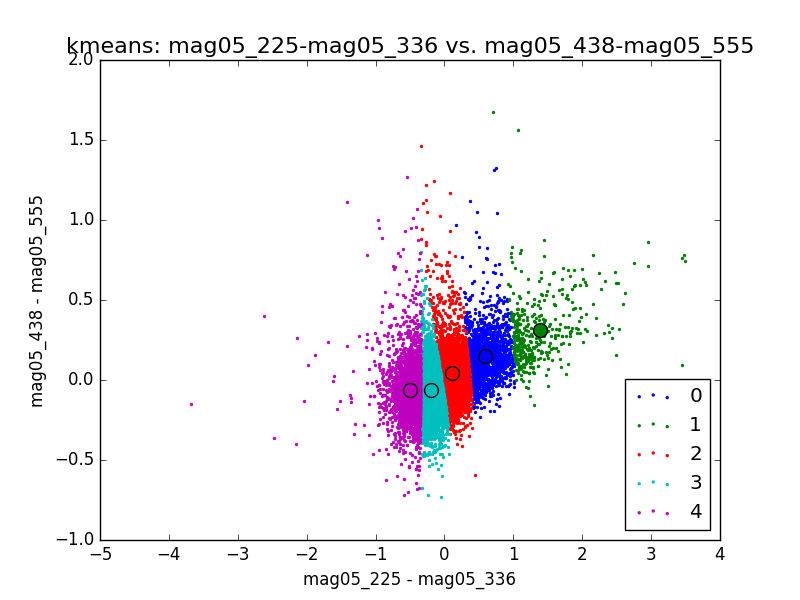
\includegraphics[width=\linewidth]{figs/kmeans_xy_5cl_mag05_225-mag05_336vsmag05_438-mag05_555}
\caption{Colour-Colour distribution of the UVW-U and B-V colours, clustered using K-Means with $K=5$. The colour of each point corresponds to the cluster the point was assigned to. Cluster numbers can be seen in the legend.}
\label{fig:UVWKM1}
\end{figure}
The algorithm split the data into groups based on its UVW - U colour. The pattern continued for all values of K, and the S Scores of the combination elbowed at $K=5$.
The second type of result for K-Means can be seen in Figure ~\ref{fig:UVWKM2}, against the B-I colour. 
This clustering segmented the data into circular groups within the distribution. 
Similar to the B-V combination, the S Score elbowed at $K=5$. 
When the objects were plotted on the whitelight image, both types of segmentation seemed to pick out objects that live in different structures of M83. % Reference Chandar
% Add test with CLAsPS score to show correlation with labels 
\begin{figure}[H]
\centering
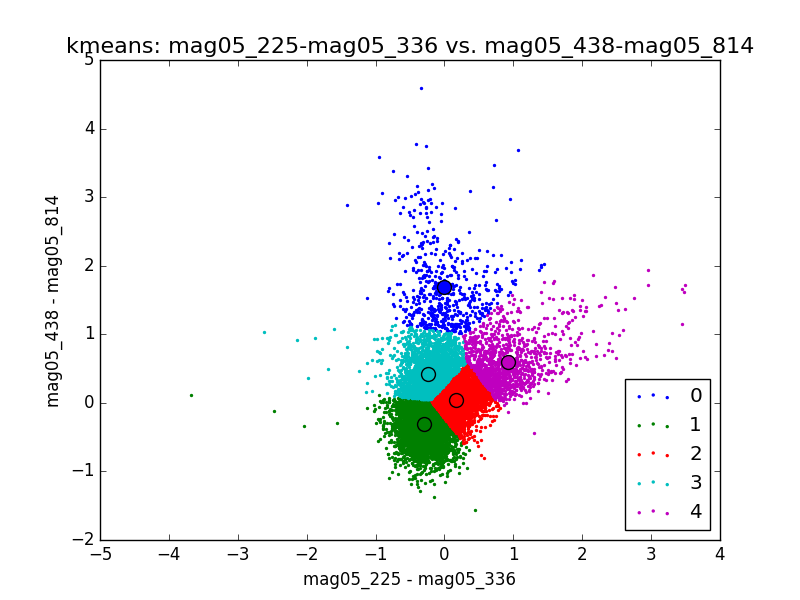
\includegraphics[width=\linewidth]{figs/kmeans_xy_5cl_mag05_225-mag05_336vsmag05_438-mag05_814}
\caption{Colour-Colour distribution of the UVW-U and B-I colours, clustered using K-Means with $K=5$. The colour of each point corresponds to the cluster the point was assigned to. Cluster numbers can be seen in the legend.}
\label{fig:UVWKM2}
\end{figure}

\subsubsection{U - OII}
The U - OII combination was clustered with the B-V, B-I, and V-I colours. % More general information about what we are looking for in this combination

\paragraph{Mean-Shift}
This colour seemed to be much more sensitive to bandwidth selection than other combinations.
With the B-V colour, $h=0.2$ produced $32$ clusters, while $h=0.4$ produced $3$. With the V-I colour, $h=0.35$ produced $17$ clusters, while $h=0.6$ produced $3$.
Due to this sensitivity, the bandwidth hierarchy was created on much narrower increases in $h$, which produced more meaningful clusters.
Using the silhouette score, the most accurate clustering produced between 3 and 6 clusters depending on the broad-broad colour used.
Two-dimentional clustering was generally more accurate for the meanshift algorithm using the silhouette score, however using three dimensions allowed the algorithm to pick out more features in the distribution. 
The three-dimensional distribution was created by using the OII band as a base, and creating colours from the other three bands in the combination. For example, the U - OII, B - V combination became: U - OII, OII - B, OII - V.
This revealed more information about the distribution of objects in that colour space, and more features for the algorithms to identify.
Despite this, meanshift still created a single, large cluster with several smaller ones. However, the borders of the clusters seemed to follow the features of the distribution more clearly using three dimensions.

\begin{figure*}
\centering
\subfloat[3D Mean-Shift Clustering: U - OII, OII - V, OII - I.]{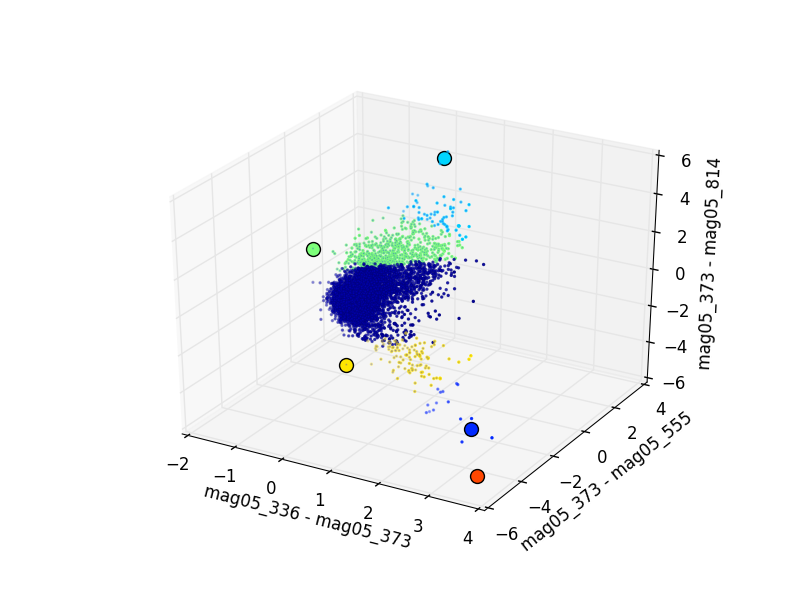
\includegraphics[width=0.5\textwidth]{figs/meanshift_3d_color_6cl_mag05_336-mag05_373vsmag05_373-mag05_555vsmag05_373-mag05_814}\label{fig:OII_3MSa}}
\hfill
\subfloat[Narrow filter distribution.]{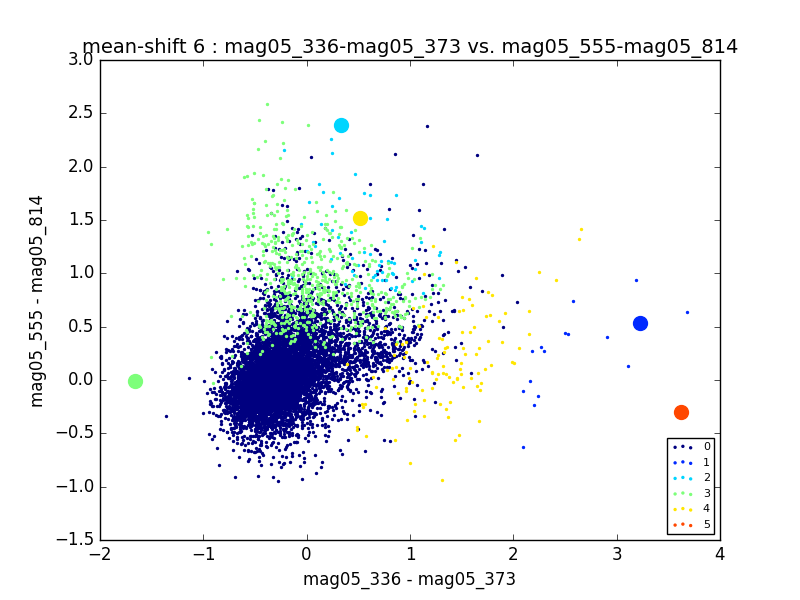
\includegraphics[width=0.5\textwidth]{figs/meanshift_base_color_6cl_mag05_336-mag05_373vsmag05_555-mag05_814}\label{fig:OII_3MSa}}
\caption{2D projection into U - OII, V - I space of 3D Mean-Shift clustering.}
\label{fig:OII_3DMS}
\end{figure*}

\paragraph{K-Means}
The K-Means algorithm was more accurate using three dimensional clustering. 
The segmentation was more effective as the algorithm was able to clearly identify different structures in the distribution. 
In two dimensions, the algorithm seemed to arbitrarely slice the distribution, instead of finding structure.
The silhouette score was always higher in three dimensions, and the score clearly peaked at a specific value of K.

\begin{figure*}
\centering
\subfloat[3D K-Means Clustering: U - OII, OII - V, OII - I.]{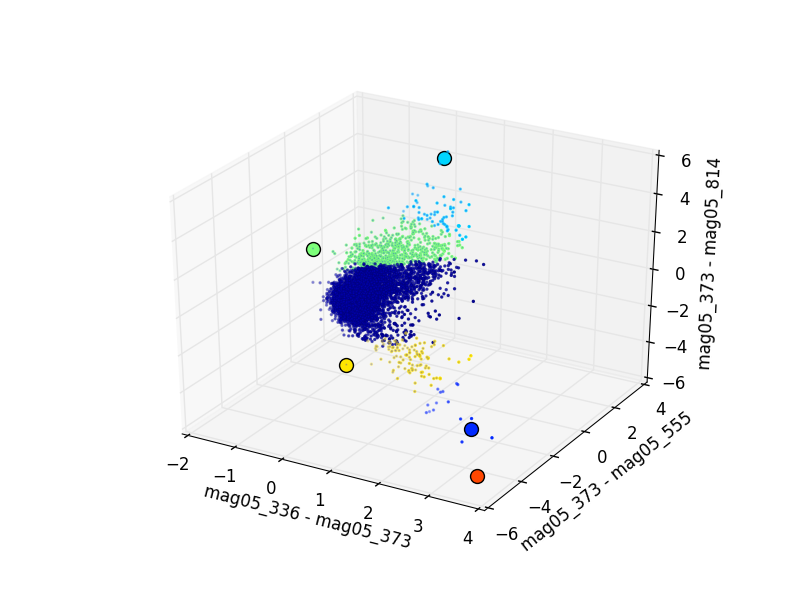
\includegraphics[width=0.5\textwidth]{figs/meanshift_3d_color_6cl_mag05_336-mag05_373vsmag05_373-mag05_555vsmag05_373-mag05_814}\label{fig:OII_3MSa}}
\hfill
\subfloat[Narrow filter distribution.]{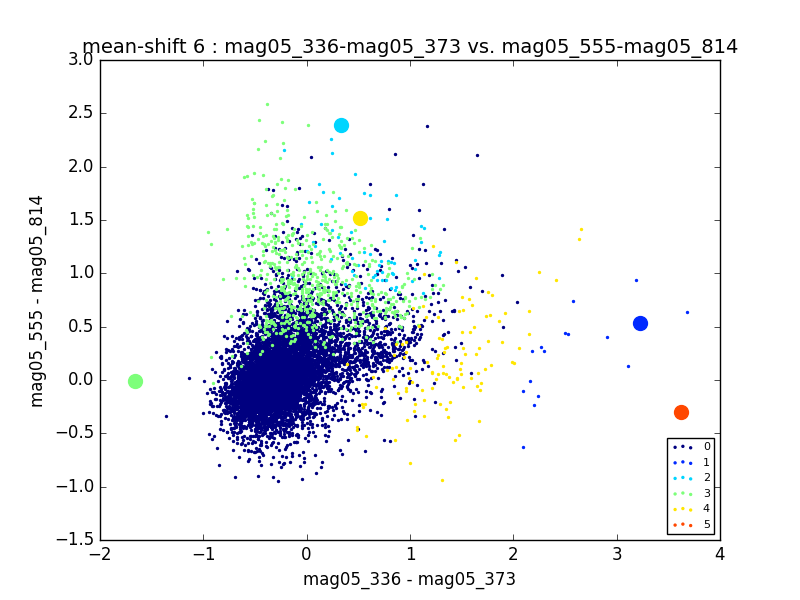
\includegraphics[width=0.5\textwidth]{figs/meanshift_base_color_6cl_mag05_336-mag05_373vsmag05_555-mag05_814}\label{fig:OII_3MSa}}
\caption{2D projection into U - OII, V - I space of 3D Mean-Shift clustering.}
\label{fig:OII_3DMS}
\end{figure*}













%\section{Discussion}
%% Discussion

\textbf{This should be where we present a process for future surveys.}
%
%\section{Summary}
%\documentclass{article}
\usepackage{graphicx}
\usepackage{sidecap}
\usepackage{epstopdf}

\begin{document}
\title{Summary of Initial Papers} 
\author{Alexander K. Kiar\\Department of Physics \& Astronomy\\Western University\\ \texttt{akiar@uwo.ca}}
\maketitle 

\begin{abstract}
Summary of questions and findings from the eight initial papers from May 27, 2016.
\end{abstract} 

\section{Eight-Dimensional Mid-Infrared/Optical Bayesian Quasar Selection} 
Explored multi-dimensional, multiwavelength selection of quasars from the IRAC and SDSS. 
Selection traditionally in two-colour space, used a combination of 8-D and 4-D techniques. 
Used Bayesian selection techniques and completness and contamination to evaluate selection.  
\begin{enumerate}
\item Converted between Vega and AB photometry
\item IRAC channels: 3.6, 4.5, 5.8, 8.0
\item Made 8 unique colours with ugriz magnitudes 
\item Used all SDSS filters and two short-wave IRAC bands 
\item Bayesian selection section 3
\item Used mean colours to classify types of quasars. Can we use that in our classification? 
\item Set colour limits to reduce error and removed faint and saturated objects. sec 3.1. Can we do the same? 
\item Can we use completeness and contamination? Need a training set, could use a set of points from the data? 
\end{enumerate}

\section{Towards auto classification of all WISE sources}
Applied support vector machines with a training sample to spectroscopic dataset to auto classify objects. 
\begin{enumerate} 
\item used four infrared bands 3.4 - 23 um 
\item used signal to noise 2 in shorter wavelengths and deteriorates in longer. 
\item significant work on colour colour space for WISE survey 
\item used magnitude, color, and differential aperture mag space 
\item computed completeness and contamination for training set. 
\end{enumerate} 

\section{Meaning of WISE colours} 
Colour magnitude criteria to select AGB stars with dust shells and seperate into classes. 
\begin{enumerate} 
\item colour plots showing distribution of object types in survey 
\item set magnitude limits to isolate certain objects. sec 2. 
\item heat map distributions of colors 
\item chose 12 colours, only 3 independent. Used the 3 to classify objects
\item use two-sided Kolmogorov Smirnov test to test distribution hypothesis. Sec 3.3.4
\item created model to predict object type based on colour
\end{enumerate} 

\section{CLaSPS: new method for knowledge extraction} 
Using unspurvised clustering to identify correlations among astronomical obersvations. 
\begin{enumerate} 
\item use combination of features and labels. We have colour features for objects, could we use labels as well? 
\item use a score and fraction of objects similar to our summary. 
\item use Kmeans and vary number of clusters applied to data set
\end{enumerate}

\end{document}


\section*{Acknowledgments}

go here.

\bibliographystyle{mn2e}
\bibliography{reference}{}

\bsp



\appendix

\label{lastpage}

\end{document}

% 2- column table
%\begin{table*}
% \centering
% \begin{minipage}{140mm}
%  \caption{Data on the RV Tauri stars detected by {\it IRAS}.}
%  \begin{tabular}{@{}llrrrrlrlr@{}}
%  \hline
%   Name     &            & \multicolumn{4}{c}{Flux density (Jy)%
%   Variable & {\it IRAS} & 12$\,\umu$m & 25$\,\umu$m & 60$\,\umu$m
%     & 100$\,\umu$m & Sp. & Period & Light- & $T_0\,(\rmn{K})$ \\
%  \hline
% TW Cam & 04166$+$5719 & 8.27 & 5.62 & 1.82 & $<$1.73 & A & 85.6 & a & 555 \\
% RV Tau & 04440$+$2605 & 22.53 & 18.08 & 6.40 & 2.52 & A & 78.9 & b & 460 \\
% DY Ori & 06034$+$1354 & 12.44 & 14.93 & 4.12 & $<$11.22 & B & 60.3 &  & 295 \\
% CT Ori & 06072$+$0953 & 6.16 & 5.57 & 1.22 & $<$1.54 & B & 135.6 &  & 330 \\
% SU Gem & 06108$+$2734 & 7.90 & 5.69 & 2.16 & $<$11.66 & A & 50.1 & b & 575 \\
% UY CMa & 06160$-$1701 & 3.51 & 2.48 & 0.57 & $<$1.00 & B & 113.9 & a & 420 \\
% \hline
%\end{tabular}
%\end{minipage}
%\end{table*}

